\documentclass{article}
\usepackage[letterpaper,top=2cm,bottom=2cm,left=3cm,right=3cm,marginparwidth=1.75cm]{geometry}

\usepackage{amsmath}
\usepackage{graphicx}
\usepackage[colorlinks=true, allcolors=blue]{hyperref}
\usepackage{listings}

\begin{document}
\begin{titlepage}
\centering
\begin{figure}
\centering
{\bfseries\LARGE Escuela técnica superior\par}
{\scshape\Large Facultad de Ingeniería Informática\par}
\vspace{5cm}
\centering
 
\includegraphics[scale=0.1]{img/logo.png} 

\end{figure}


{\scshape\Huge Práctica 7\par}
{\scshape\Large  Scripts de bash\par}
\vspace{9cm}
{\Large Ignacio Fernández Contreras\par}
\vfill
\end{titlepage}
\clearpage\hbox{}\thispagestyle{empty}\newpage

\section{Parte 1}
Resuelva los siguientes ejercicios de clase.
\subsection{Ejercicio 1.}
Escriba un script que haga lo siguiente:
\begin{itemize}
\item Compruebe que se le pasa al menos un parámetro, en caso contrario
termina (return) el script con código 1.
\item Compruebe que se le pasa un directorio como argumento, en caso
contrario termina con código 2.
\item Si se le pasa un directorio, debe comprobar que no es el directorio
actual y que tiene permisos de búsqueda, en caso contrario devuelve
el código 3. En caso afirmativo, nos desplazamos hacia él.
\end{itemize}
Notas:
\begin{itemize}
\item Ejecuta este script con source o ‘.’ 
\item La variable $\$$PWD nos devuelve el directorio actual.
\end{itemize}

\begin{center}
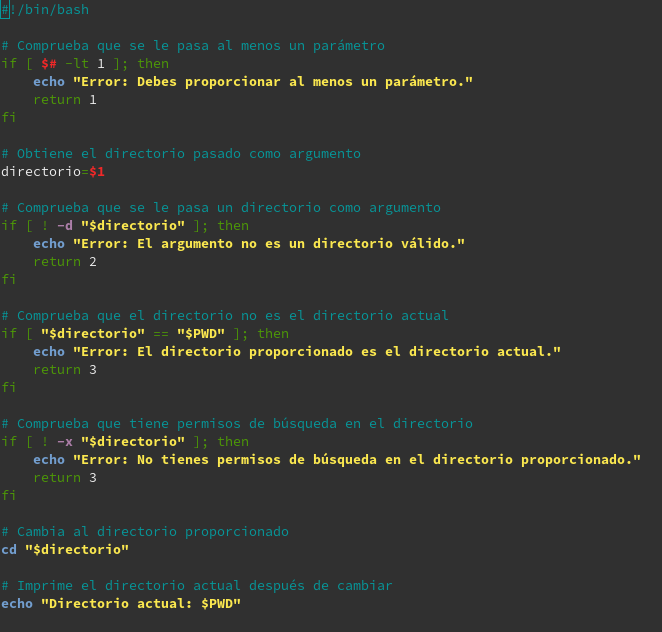
\includegraphics[width=\textwidth]{img/img1.png} 
\end{center}

\begin{center}
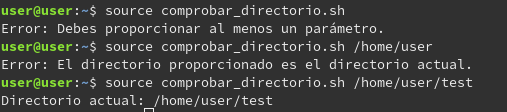
\includegraphics[width=\textwidth]{img/img2.png} 
\end{center}

\subsection{Ejercicio 2.}
Extienda el script anterior para que liste todos los ficheros
ejecutables que haya en el directorio pasado como argumento.

\begin{center}
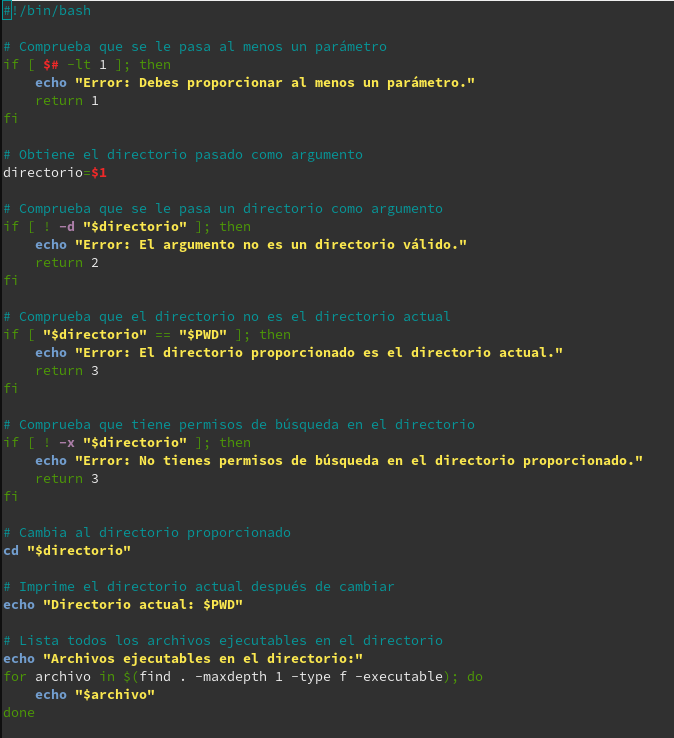
\includegraphics[width=\textwidth]{img/img3.png} 
\end{center}
\begin{center}
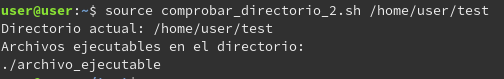
\includegraphics[width=\textwidth]{img/img4.png} 
\end{center}

\subsection{Ejercicio 3.}
Sabiendo que el operador $\$\{\#var\}$ devuelve el tamaño de una
cadena, y utilizando el operador para obtener una subcadena
$\$\{var:offset:longitud\}$, cree una función Reverse que devuelva a través de
variable global una cadena de caracteres invertida. 

\begin{center}
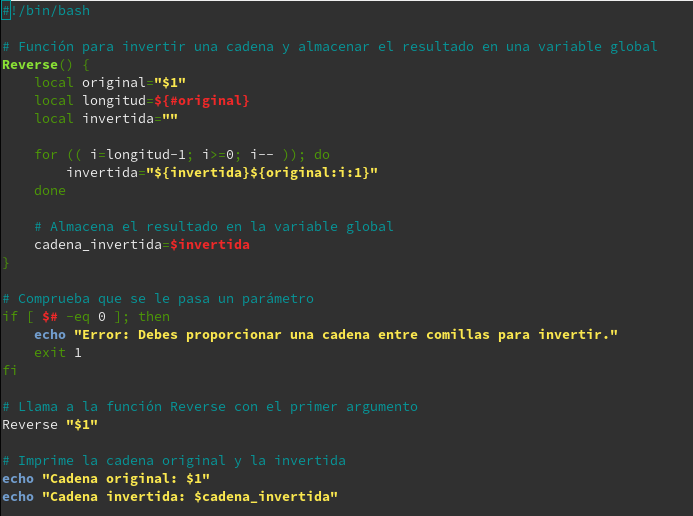
\includegraphics[width=\textwidth]{img/img5.png} 
\end{center}
\begin{center}
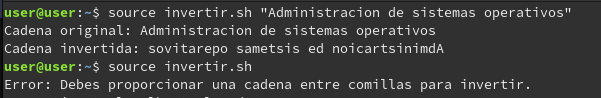
\includegraphics[width=\textwidth]{img/img6.png} 
\end{center}

\newpage


\section{Parte 2}
Explica paso a paso el siguiente script de bash:

\lstset{language=C, breaklines=true, basicstyle=\footnotesize}
\begin{lstlisting}[frame=single]
function ZZZ {
IFS='
'
	ficheros=$(ls -1 $1)
	for fichero in $ficheros
	do
		path_fichero="$1/$fichero"
		if [ -x $path_fichero ]; then
			echo $path_fichero
		fi
	done
	IFS=':'
}

IFS=':'
for dir in $PATH
do
	if [ -z "$dir" ]; then
		echo "ENCONTRADO UN DIRECTORIO VACIO"
		exit 1
	elif ! [ -d "$dir" ]; then
		echo "$dir NO ES UN DIRECTORIO VALIDO"
		exit 1
	else
		ZZZ $dir
	fi
done
\end{lstlisting}


\begin{itemize}
\item Función ZZZ
\begin{itemize}
\item Se añade una simple línea delante del for para que no trate los espacios como separador y obtengamos el listado como queremos
\item Obtiene la lista de archivos en el directorio proporcionado ($\$$1) y la almacena en la variable ficheros.
\item Itera sobre cada archivo en ficheros y verifica si es ejecutable.
\item Imprime la ruta completa de los archivos ejecutables encontrados.
\end{itemize}
\item Bucle principal
\begin{itemize}
\item añadir una simple línea delante del forpara que no trate los : como separador y obtengamos el listado como queremos
\item Itera sobre cada directorio en PATH.
\item Verifica si el directorio es una cadena vacía y, si es así, imprime un mensaje de error y sale del script con el código de salida 1.
\item Verifica si el elemento en PATH no es un directorio válido, imprime un mensaje de error y sale del script con el código de salida 1.
\item Si el directorio es válido, llama a la función ZZZ con el directorio como argumento.
\end{itemize}
\end{itemize}

\newpage


\section{Ej 3}
La sucesión alícuota es una sucesión de números que resulta de la suma de
los divisores propios del término anterior. La sucesión da comienzo en un
término k mayor que 0 y termina cuando se alcanza el término 1. En caso de
que se repita el término anterior o se alcancen más de 10 términos, se
considera una sucesión alícuota infinita y se para la serie. A continuación, se
muestra varios ejemplos de sucesiones alícuotas:


\begin{center}
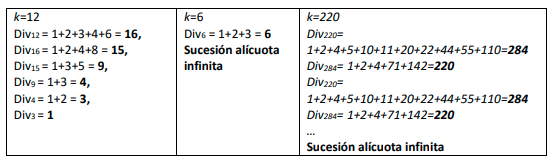
\includegraphics[width=0.8\textwidth]{img/img9.png} 
\end{center}


Escriba un script de bash que lea un término k mayor que 0 desde teclado y
muestre la sucesión alícuota de dicho término. En el caso de una sucesión
alícuota infinita, cuando se detecte, se mostrará un mensaje indicándolo. A
continuación, se muestran varios ejemplos de la ejecución del programa:

 
\begin{center}
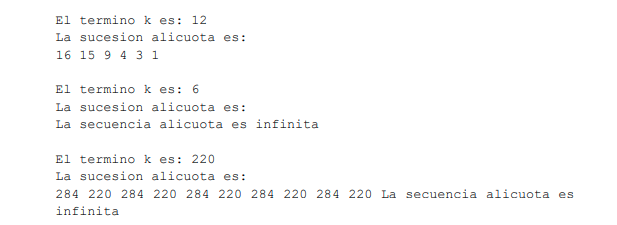
\includegraphics[width=0.8\textwidth]{img/img10.png} 
\end{center}


\begin{center}
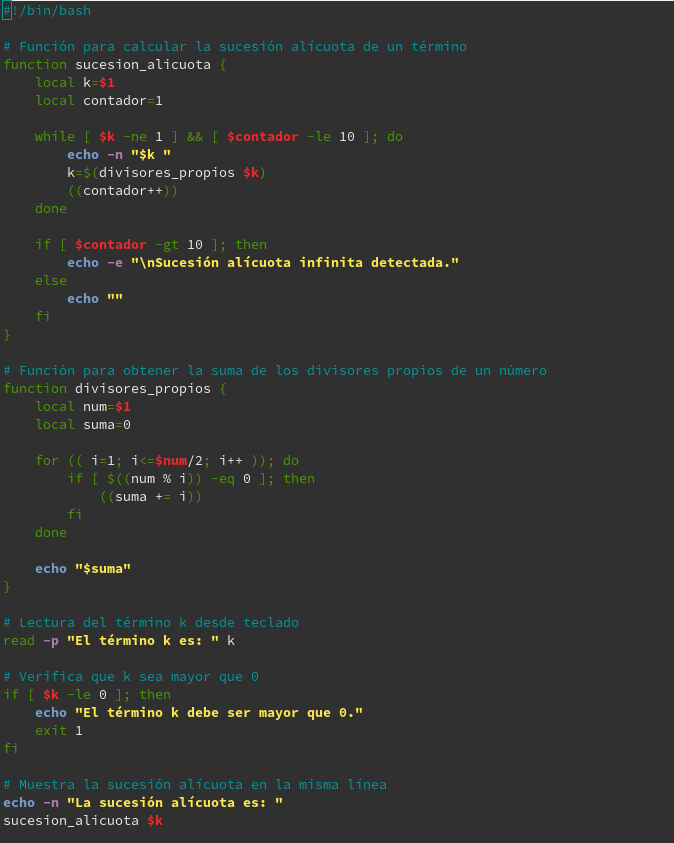
\includegraphics[width=\textwidth]{img/img7.png} 
\end{center}


\begin{center}
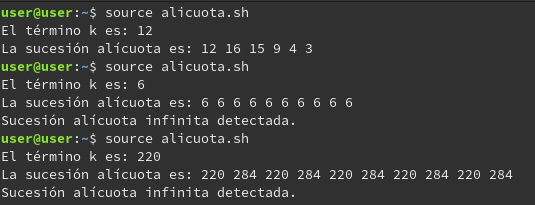
\includegraphics[width=\textwidth]{img/img8.png} 
\end{center}






\end{document}
